

\newtheorem*{remark}{}
\newtheorem*{definition}{Definition}

\mychapter{1}{Mathematical Base to Cryptography}
\begin{center}
	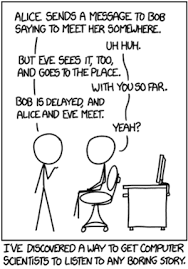
\includegraphics{Photos/chapter_cover_1.png}
\end{center}

	
	\mysection{1}{Introduction to Cryptography}

		\subsection{Some terminologies}
		\begin{itemize}
			\item \emph{Plaintext,} The message, usually alphabetic in this context, that you wish to send. \\ Depicted using small letters \(a\), \(b\), \(c\), \( \cdots \) 

			\item \emph{Ciphertext,} The message that will be transmitted after enciphering. \\ Depicted using captial letters \(A\), \(B\), \(C\), \(\cdots\)

			\item \emph{Key,} The word/ phrase/ alphabetic order using which we encrypted our \emph{Plaintext}.

			\item \emph{Monoalphabetic Substitution Cipher,} A cipher key which uses only one set of alphabet to encrypt the \emph{Plaintext}

			\item \emph{Polyalphabetic Substitution Cipher,} A key that consists of multiple alphabetic orders/  keywords to encrypt the message.  

			\item \emph{Alice, Bob and Eve,} The quintessential trio studied in Cryptology examples wherein \emph{Alice} and \emph{Bob}, are trying to communicate secretly which \emph{Eve} tries to intercept and decrypt the messages.
		\end{itemize}

	 	\subsection{Early Cryptography}
	 		The earliest forms of monoalphabetic\footnote{Consisting of only 1 key} ciphers include the \emph{Caesarean/Shift Cipher}. This involves shifting of the alphabet by a few (historically 3) letter to encrypt the \emph{Plain text.} \\
	 		This yields us with only 26 possible cipher keys which can be easily cycled through by Eve, once she is sure that Caeser Cipher has been used, hence providing us with next none security. \par
	 		Of course, there exist a very large number of random monoalphabetic cipher keys (\(26! \approx 4\times10^{26}\) to be precise) but monoalphabetic ciphers can be easily broken into using statistical analysis of the cipher text. Tools employed by cryptanalysts include- 
	 		\begin{itemize}
	 			\item Frequency of letters
	 			\item Frequency of Bigrams (pairs of letters that occur together)
	 			\item Presence of vowels 
	 		\end{itemize}
	 		\begin{mybox}Another classical cipher, which used polyalphabetic cipher keys, \emph{Vigen\`{e}re} cipher will be analysed in later weeks.\end{mybox}
	 
	 \begin{mdframed}
	 \mysection{2}{Some Mathematical Pre-requisites for Modular Arithematic}
	 	\subsection{GCD}\label{subsec:gcd}
	 		\begin{definition}\label{def:Euclid}
	 			\emph{GCD} of any 2 integers is the largest positive integer that divides each of the integers, provided both integers aren't 0.
	 		\end{definition}
	 		The standard procedure to find \(\gcd(a,b)\) is to list out factors of \(a\) and \(b\), and choose the largest factor common to both. But an even faster algorithm exists called the \emph{Euclid's algorithm}. It uses the fact that \(\gcd(a,b)=\gcd(a-k \cdot b, b), \forall a,b,k \in \mathbb{Z}\) such that \( a>b\)\footnote{Proof: Suppose you have 2 numbers \(a, b\) such that \(\gcd (a,b) = g\) thus we can write \(a = p \cdot g\) and \(b = q \cdot g\). Obviously then, if we defined \(c = a-b= (p-q) \cdot g\), will have \(g\) as a divisor. \\ Futhermore, let us denote \(\gcd(b,c)=h\). Thus we can also write \(b = m \cdot h\) and \(c = n \cdot h\). Upon rearranging, we get \(a=b+c=(m+n)\cdot h\) which tells us clearly that \(h\) will have to be a divisor of \(a\).\\ Now, at this point, all of \(a, b\) and \(c\) have both \(g\) and \(h\) as factors. So the only way \(\gcd(a,b)\) does not exceed the initially set \(g\) is because \(g = h\). \textcolor{orange}{Tada!}} \par
	 		Thus to find \(\gcd(A,B)\), we can use this algorithm
	 		\begin{enumerate}
	 			\item Take $a=A$, $b=B$
	 			\item If $b>a$, swap them.
	 			\item \(\gcd(a, b)=\gcd(a-k \cdot b, b)\) so replace \(a\) with \(a-k \cdot b\) such that \((k+1) \cdot b > a\) and \(k \cdot b < a\)
	 			\item If \(a=0\), \(\gcd(A,B)=b\) \\ else swap $a$ and $b$, and repeat from Step 3. 
	 		\end{enumerate}
	 		\textbf{Some interesting results-}
	 		\begin{itemize}
	 			\item \(r_{n+2}<\frac{r_n}{2}\) where \(r_n\) is the $n^{th}$ remainder\footnote{Proof- Assuming 2 cases (1. \(r_{n+1}<\frac{r_n}{2}\) is obvious,2. \(r_{n+1}>\frac{r_n}{2}\) ensures that \(r_n=1.r_{n+1}+r_{n+2} \Rightarrow r_{n+2}=r_n-r_{n+1}<\frac{r_n}{2}\))}.
	 			\item it takes at most \(2 \log_{2}{b} +2\) steps\footnote{We can use the fact that if \(b \in [2^{n-1}, 2^n)\) and \(r_{2k+1}<\frac{b}{2^{k}}\), we can easily see that this is true since \(2n+1=2(n-1)+2<2 \log_{2}{b} +2\) }.
	 			\item We can prove that \(\gcd(a,b)=u \cdot a + v \cdot b\) where \(u, v \in \mathbb{Z}\). These \(u, v\) values can be determined using a simple algorithm if we know the quotients at each step. \\
	 			We can even find the original \(a\) and \(b\) if we have all the quotients.
	 			\item The above statement also means that if \(\gcd(a,b)=1\), we can write any number using linear combinations of \(a\) and \(b\). 
	 		\end{itemize}
	 \end{mdframed}
	 
	 \mysection{3}{Modular Arithematic}
	 	\subsection{Format}
	 		\centering \(a \equiv b \bmod(m)\) where \(a-b\) is divisible by $m$ \par
	 		\raggedright  
	 	
	 	\subsection{Properties}
	 	\begin{itemize}
	 		\item If \(a \cdot b \equiv 1 \bmod(m)\ \exists b \in \mathbb{Z} \iff \gcd(a,m)=1\), we say that $b$ is the \emph{modular inverse} of $a$ modulo $m$. \\
	 		\emph{\underline{Note-} Although multiple values of $b$ will exist if \(\gcd(a,m)=1\), all will have the same value of \(b \bmod(m)\). Hence we used the term \textbf{the inverse}.}
	 		\item If \(a_1 \equiv b_1 \bmod(m)\) and \(a_2 \equiv b_2 \bmod(m)\), then, \(a_1 \cdot a_2 \equiv b_1 \cdot b_2 \bmod(m)\)
	 		\item We can denote \emph{inverse} of $a$ as \(a^{-1}\) such that, \(a^{-1} \equiv b \bmod(m)\). \\
	 		Hence \(7^{-1} \equiv 8 \bmod(11)\). This means if we can write \(\frac{4}{7} \equiv 7 \cdot 8 \bmod(11) \equiv 1 \bmod(11)\) as \(4 \equiv 7 \bmod(11)\). \\
	 		\emph{The interesting thing to note here is that it isn't easy to find the modular inverses of numbers as \(m\) becomes larger.}
	 		\item Since we can write \(a \cdot b \equiv 1 \bmod(m)\) as \(a \cdot b= q \cdot m + 1\), from the result obtained in last section, we can be sure that finding a value of b will take no. of steps \(\sim \log_{2}m\).
	 	\end{itemize}

	 	\begin{tcolorbox}
	 		You might think that finding the modulo of products of large numbers might take the same amount of time as it takes for calculating the product but you can easily cut down time on it. \\ Example- \(170242 \times 261494 \bmod(10) \equiv 2 \times 4 \equiv 8 \bmod(10)\). Hence it is \textcolor{red}{\textbf{\underline{\emph{FAST}}}}.
	 	\end{tcolorbox}

	 	\subsection{Ring theory}
	 		As we can see in the above definitions, it is obvious that in \(a \equiv r \bmod(m)\), \(r \in [0, m-1] \cap \mathbb{Z}\). We can then say that \(r \in \mathbb{Z}/ m \mathbb{Z}\) where \(\mathbb{Z}/ m \mathbb{Z}\) is the ring of integers with modulo \(m\). \par
	 		\indent For addition and multiplication in \(\mathbb{Z}/ m \mathbb{Z}\) space, we just divide the answer with \(m\) and use the remainder as final value.
	 		\\
	 		\noindent \emph{Units modulo m-} If \(\gcd(a,m)=1\), OR \(a^{-1}\) exists for modulo \(m\), we say that $a$ is units modulo $m$. 
	 		\begin{itemize}
	 			\item If \(a_1, a_2\) are units modulo \(m\), \( a_1 \cdot a_2 \) will also be a units modulo \(m\).
	 			\item If \(a_1, a_2\) are units modulo \(m\), \( a_1 + a_2 \) need not be a units modulo \(m\).
	 		\end{itemize}
	 		The set \(\ast(\mathbb{Z}/ m \mathbb{Z})\) is called the group of units modulo \(m\) and can also be defined as-
	 		\centering \(\ast(\mathbb{Z}/ m \mathbb{Z})={a\in \mathbb{Z}/ m \mathbb{Z}, \gcd(a,m)=1}\)
	 		\raggedright If we took a subset of units modulo \(m= \textbf{P}\), then-
	 		\begin{itemize}
	 			\item If \(k_{i,j}= a_i \cdot a_j,\) where \(a_i, a_j \in \textbf{P},\) then \(k_{i,j}\) also belongs to \(\textbf{P}\).
	 			\item If \(k_{i,j}= a_i + a_j,\) where \(a_i, a_j \in \textbf{P},\) then \(k_{i,j}\) need not belong to \(\textbf{P}\).
	 		\end{itemize}
	 		\textbf{Euler's Totient/ Phi Function-} \(\phi(m)=\# \ast(\mathbb{Z}/ m \mathbb{Z})\) OR $\phi(m)$ counts the number of \(a \in [1,m-1]\), such that, \(\gcd(a,m)=1\) i.e. number of values of \(a<m\) such that \(a\) and \(m\) are co-prime\\
	 		\emph{e.g. \(\phi(24)=8, \phi(7)=6\)} \\ \emph{\underline{Note-} Notice how \(\phi(p)\) where \(p\) is a prime number, will always be \(p-1\)}

	 	\subsection{Shift Ciphers and Modulo Arithematic}
	 		We can assign numbers from 0 through 25 to all the letters in the alphabet and then use modulo arithematic for encryption and decryption-
	 		\begin{itemize}
	 			\item For a shift of \(k\), we can encrypt any letter whose number is denotes by \(p\) to a letter \((p+k) \bmod(26)\)
	 			\item To decrypt the cipher text (\(p'\)), you subtract in the ring via \((p'-k) \bmod(26)\).
	 		\end{itemize}
	 	\subsection{Fast Powering algorithm}\label{subsec:fastexpo}
	 		To calculate \(g^A \bmod(m)\), where \(g, A \in \mathbb{N}\), it can take \(\sim 2^n)\) multiplications if \(A \in [2^n, 2^{(n+1)})\). We can, however, use the fact that $g$ can we written as a linear combination of powers of 2 to reduce the number of steps we take.
	 		\begin{itemize}
	 			\item Express \(A=\sum_{n=0}^{k}{a_r 2^r}\) where \(2^k \leq A < 2^{(k+1)}\)
	 			\item Let \(g_r = g^{2^r}\). We can find \(g_1\) using \(g \cdot g\) and for subsequent values of r, we can just use \(g_{r+1} = g_r \cdot g_r\)
	 			\item Now we have \(g^A = 
	 			\sum_{r=0}^{k}{g^{a_0 + a_1 \cdot 2 + a_2 \cdot 2^2 +\cdots}}=
	 			\sum_{r=0}^{k}{g_0^{a_0}+ g_1^{a_1} + \cdots}\)
	 			\item \(x^2 \bmod(N) = (x \bmod(N))^2 \bmod(N)\)
	 		\end{itemize}
	 		Keep in mind that \(a_r\) can only take the values 0 and 1 thus we can say that this method takes \(2r\) multiplication steps at most. (Including the exponential expansion of \(A\)).
	 \mysection{4}{Prime numbers and Finite Fields}\label{sec:prime}
	 	\subsection{Division modulo $m$}
	 		We can usually do multiplication, subtraction, addition modulo \(m\) but division modulo \(m\) is only possible if the divisior(\(k\)) is coprime with \(m\). \par
	 		\noindent \emph{Divison modulo \(m\) means- If \(a=p\bmod(m)\) and \(b=q \bmod(m)\),} \par
	 		\centering\emph{\(c= \frac{a}{b}= \frac{p'}{q'}\)} \par
	 		\raggedright where \(p \bmod(m) = p' \bmod(m)\) and \(q \bmod(m) = q' \bmod(m)\) and \(\frac{p'}{q'} \in \mathbb{Z}\). It is only possible if \(\gcd(b,m)=1\) as otherwise you cannot get a unique value. \\
	 		Example- \(a= 11 \bmod (5)\), \(b = 4 \bmod (5)\) then \(\frac{a}{b}= \frac{11 \bmod (5)}{4 \bmod (5)}=\frac{16 \bmod (5)}{4 \bmod (5)}\)=4\\
	 		\emph{Note-} In the above example, 4 is the only integral value possible of \(\frac{a}{b}\). Values such as \(\frac{11 \bmod(5)}{4 \bmod(5)}=\frac{1}{4}\) are ignored. \par

	 		The reason for \(\gcd(4, 5)=1\) being necessary in the above examples is that we can write \(\frac{11 \bmod(5)}{4 \bmod(5)}= 11 \cdot 4^{-1} \bmod(5)\) and \(4^{-1}\) can only exist if \(\gcd(4,5)=1\). (Here \(4^{-1}= 4\) thus our answer = \(44 \bmod (5)=4\))

	 	\subsection{Division in rings}
	 		As seen earlier, if \(\gcd(a,m)=1\), we can easily divide modulo \(m\) by a any integer. If we now studied rings of form \(\mathbb{Z}/p\mathbb{Z}\), where \(p \in prime\) we will get that any integer \(b\in \mathbb{Z}/p\mathbb{Z}\) can be used in division as obviously \(b<p\) AND \(p\in prime\) thus \(\gcd(b,p)=1\) \par
	 		
	 		\begin{mybox}\label{theo:extendedEuclid}
	 			\underline{Note-} If \(a\in\ast\mathbb{Z}/m\mathbb{Z}\), \(a\) can be used as a divisor modulo $m$. ALSO \(\mathbb{Z}/p\mathbb{Z}\)= \(\ast \mathbb{Z}/p\mathbb{Z}\). \par
	 			\emph{We can calculate \(a^{-1}\) using- \(au+pv=1\) (as \(\gcd(a,p)=1\)), wherein solving for $u$ yields us \(a^{-1} \bmod(p)\).}
	 			\tcblower
	 			The last line is the \textbf{Extended Euclidean Theorem}. Unlike the normal \hyperref[def:Euclid]{Euclid's theorem}, the easiest way to describe its working is via a \hyperref[add:codeForRecursive]{recursive C code}.
	 		\end{mybox}

	 	\subsection{Finite Fields}
	 		Since we can compute division, addition, multiplication and subtraction in \(\mathbb{Z}/p\mathbb{Z}\), we can call it a field just like \(\mathbb{R}/\mathbb{Z}/\) etc\(\cdots\) \\
	 		Since \(\mathbb{Z}/p\mathbb{Z}\) only has a finite number of elements, we call it a finite field and can even denote it by \(\mathbb(F)_p\) to show the finitedness.
	 \mysection{5}{Fermat's ``Little'' Theorem}\label{sec:fermat}
	 	The theorem states that- \par
	 	\centering \(a^{p-1} \equiv 1 \bmod(p)\) for \(a \not = k \cdot p\) \par
	 	\begin{mdframed}
		 	\raggedright \textbf{Proof:} \\
		 	Since \(a \not= k \cdot p\), \(a, 2a, 3a, 4a, \cdots (p-1)a \bmod(p) \not= 0\). Now if we considered \(k \in [1,p-1]\), \par
		 	\centering \(k_1 \cdot a \equiv j_1 \bmod(p)\) AND \(k_2 \cdot a \equiv j_2 \bmod(p)\) \par
		 	\(\Rightarrow (k_1-k_2)\cdot a \equiv (j_1-j_2) \bmod(p)\) \par
		 	\raggedright Since \(k_1 - k_2\) cannot be a multiple of \(p\), \(j_1 - j_2 \not= 0\) and so for every \(k \in [1, p-1]\), we get a distinct \(j \in [1, p-1]\). Hence we get a bijective function of \([1,p-1] \rightarrow [1,p-1]\). So- \par
		 	\centering \( \prod_{k=1}^{p-1}k \cdot a \equiv  \prod_{k=1}^{p-1}{k} \bmod(p) \Rightarrow (p-1)! a^{p-1} \equiv (p-1)! \bmod(p)\) \par
		 	\(\Rightarrow a^{p-1}=1 \bmod(p)\)
	 	\end{mdframed}
	 	\raggedright We can use this to find the inverse of any number modulo \(p\)- \\ \centering \(a\cdot a^{p-2}\equiv 1 \bmod(p) \Rightarrow a^{-1} \equiv a^{p-2} \bmod(p)\) \par \par  
	 	\LARGE \emph{\textcolor{orange}{Voila!}}  \\ \tiny We just found an inutitive, new way to check if a number is composite or not \par
	 	\raggedright \small If we wanted to check if a number \(n\) was prime or not-
	 	\begin{itemize}
	 		\item If \(n \in even\), obviously composite
	 		\item If \(n\in odd\), take \(a=2\). Now if \(2^{n-1} \not \equiv 1 \bmod(n)\), we can be sure that it is definitely composite. \footnote{As is with all good things in life, this too has an asterisk- you cannot judge if a number is prime or not solely based on this. There is a subset of composite numbers called the ``Carmicheal Numbers'' which satisfy \(b^{(n-1)} \equiv 1 \bmod(n)\) despite their lack of primality. Just random gifts of joy Mathematics bestows upon you. It is better discussed in \hyperref[subsec:witness]{a later section}.} \\
	 	\end{itemize}
	 	\definition{\emph{We define} order \emph{as the smallest number \(k\) such that}} \par 
	 	\centering \(a^k\equiv 1 \bmod(p)\) \par 
	 	\raggedright \em We can also be sure that \(p-1\) is divisible by \(k\). 
		 \subsection{Primitive Roots Theorem}\label{subsec:primitive}
		 The theorem states that \emph{for a prime number $p$, there always exists a number \(g \in \mathbb{F}_p\), such that every element of \(\mathbb{F}_p^{*}\) can be expressed as a power of $g$ } \par
		 Number of primitive roots of \(p= \phi(p-1)\)
		 \begin{tcolorbox}
		 	\textbf{Example-} Let us study \(\mathbb{F}_7^*\). Since \(7 \in \text{primes}\), \(\mathbb{F}_7^* \equiv \mathbb{F}_7\). \\
		 	3 is considered a primitive root of this finite field so-
		 	\[1, 3, 3^2, 3^3, 3^4, 3^5, 3^6 \bmod(7) \equiv 1, 3, 2, 6, 4, 5, 1\]
		 	Even 5 is considered as so-
		 	\[1,5,5^2,5^3,5^4,5^5,5^6 \bmod(7)\equiv 1,5,4, 6, 2, 3, 1\]
		 	However 6 is not one-\label{example:six}
		 	\[1,6,6^2,6^3,6^4,6^5,6^6 \bmod(7) \equiv 1, 6, 1, 6, 1, 6,1\]
		 	(Note how despite 6 despite not being a primitive root, still satisfies \(6^{p-1} \bmod(p) \equiv 1\).)\\

		 	\(\phi(6)=\phi(2\times3)=1\times 2=2\) thus number of primitive roots of \(7 \equiv \phi(7-1) = 2\) 
		 \end{tcolorbox}

	\mysection{6}{Symmetric Ciphers}
		\subsection{Notations}
			If you have a message \(m \in \mathcal{M} \) (where \(\mathcal{M}\) is the list of all possible messages), you can choose a key \(k \in \mathcal{K}\) (again, where \(\mathcal{K}\) is the space of all keys), to get a cipher \(c \in \mathcal{C}\). (At this point if you cannot guess what \(\mathcal{C}\) stands for, I don't think you should read further).\par
			We thus need invertible functions \(e_k(m)\) and \(d_k(m)\) as -\par
			\centering \(e_k(m_i)= c_i\) AND \(d_k(e_k(m))=m\) \par
			\raggedright

		\subsection{Principles of Succesful Ciphers}
			\begin{mybox}
				Kerckhoff’s principle says that the security of a cryptosystem should depend only on the secrecy of the key, and not on the secrecy of the encryption algorithm itself. 
			\end{mybox}
			So keeping that in mind, we design a few principles-
			\begin{enumerate}
				\item For any plaintext \(m\) and key \(k\), it must be easy to calculate \(e_k(m)\).
				\item For any ciphertext \(c\) and key \(k\), it must be easy to calculate \(d_k(m)\).
				\item If you have ciphertexts \(c_1, c_2, c_3\cdots c_\alpha\) encrypted using the key \(k\), it should be really difficult to find \(d_k(c_1), d_k(c_2), \cdots d_k(c_\alpha)\) without knowing \(k\).
				\item If you have \(c_1, c_2, c_3, \cdots c_\beta\) and the corresponding messages \(m_1, m_2, m_3, \ldots m_\beta \), it should still be difficult to decipher a \(c\) not in this set.
			\end{enumerate}

		\subsection{Encoding of Cipher Blocks}
			We can represent any plaintext in the form of bits \(m_{B-1}m_{B-2}\cdots m_2m_1m_0\) where \(m_i \in {0,1} \forall i\in [0,B)\). Then we can break it into bytes or blocks of some other size and encode each block separately. We prefer to choose a \(\mathcal{K}\) such that \(k \in [0, 2^{B_k})\) and \(B_k \geq 80\) bits or \(160\) bits based on the message type. (This number is chosen based on the computing capacity of a modern computer since you can brute-force check each and every key \(k \in \mathcal{K}\), if \(B_k\) is not large enough.) 

		\subsection{Examples of Symmetric Ciphers}
			Choose \(\mathcal{K}=\mathcal{C}=\mathcal{M}=\mathbb{F}_p^*\) for some prime number \(p\) and then you can define- \par
			\centering \(e_k(m)\equiv k \cdot m \bmod(p)\) \par
			\raggedright Using that you can also find \(k'\) (in \(2\log_2(p)+ 2\) steps) such that- \par
			\centering \(d_k(c)\equiv k' \cdot c \bmod(p)\) to yield us \(d_k(c) \equiv m\) \par
			\raggedright Although this method follows the first 3 principles, it fails the fourth principle of successful ciphering as- \par
			\centering \(k \equiv m^{-1} \cdot c \bmod(p)\) \par 
			\raggedright The above formula gives you the exact key as soon as you find one pair of ciphertext and plaintext thus is not preferable at all.

			\subsubsection*{Simple multiplicative cipher}
				If instead of using a modulo p, if you just used \(e_k(m)= k \cdot m\), you can easily find \(\gcd(c_1, c_2, c_3 \cdots c_\alpha)\) which can give you the value of \(k\) outright. (Calculating GCD of multiple numbers is not labour intensive for a computer)

			\subsubsection*{Affine Cipher}
				Here we define ciphertext using both multiplication and addition modulo p- \par
				\[e_k \equiv k_1 \cdot m + k_2 \bmod(p)\] AND \[d_k(c) \equiv k_1' \cdot (c-k_2) \bmod(p)\] \par	
				\raggedright \emph{Note- Caesarean Shift Cipher is just a special case of this cipher with \(k_1 = 1\)} \par 

			\subsubsection*{Hill Cipher}
				In this cipher, we first denote every message of length \(n\) as a \(n \times 1\) column matrix. Then we can define a key \(k= k_{1,1}k_{1,2}k_{1,3}\cdots k_{n,n}\) as- \par 
				\[
				k=
				\begin{bmatrix}
					k_{1,1} & k_{1,2} & k_{1,3} & \dots & k_{1,n}\\
					k_{2,1} & k_{2,2} & k_{2,3} & \dots & k_{1,n}\\
					k_{3,1} & k_{3,2} & k_{3,3} & \dots & k_{1,n}\\
					\vdots & \vdots & \vdots & \ddots & \vdots \\
					k_{n,1} & k_{n,2} & k_{n,3} & \dots & k_{n,n}
				\end{bmatrix}
				\]
				We can calculate the inverse of \(k= k^{-1}\) and using the both of them, our cipher looks like-
				\[
				\begin{bmatrix}
					k_{1,1} & k_{1,2} & k_{1,3} & \dots & k_{1,n}\\
					k_{2,1} & k_{2,2} & k_{2,3} & \dots & k_{1,n}\\
					k_{3,1} & k_{3,2} & k_{3,3} & \dots & k_{1,n}\\
					\vdots & \vdots & \vdots & \ddots & \vdots \\
					k_{n,1} & k_{n,2} & k_{n,3} & \dots & k_{n,n}
				\end{bmatrix}
				\cdot 
				\begin{bmatrix}
					m_{1,1}\\
					m_{2,1}\\
					m_{3,1}\\
					\vdots \\
					m_{n,1}
				\end{bmatrix}
				=
				\begin{bmatrix}
					c_{1,1}\\
					c_{2,1}\\
					c_{3,1}\\
					\vdots \\
					c_{n,1}
				\end{bmatrix}
				\]
				Unfortunately both Affine and Hill Ciphers are both susceptible to plain text attacks. Hence we cannot use either one of these despite how dapper they look.

			\subsubsection*{XOR Cipher}
				XOR \(\oplus\) of key and message \(c \equiv m \oplus k\) seems like a good option but it has the following flaw if you have access to 2 ciphers made using the same key-
				\[
					c' \oplus c \equiv (m' \oplus k) \oplus (m \oplus k) \equiv m' \oplus m
				\]
				\begin{center}
				\begin{tabular}{c | c  c}
					 \(m\oplus m'\)&Possible $m$ &Possible $m'$\\ 
					 \hline
					 0&0&0\\
					 0&1&1\\
					 \hline
					 1&0&1\\
					 1&1&0\\
					 \hline  
				\end{tabular}
				\end{center}
				Thus we can easily find information about \(m\) from just 2 ciphers. (Although still \(m\) exactly isn't visible)

		\subsection{Random bit sequences}\label{subsec:random}
				To circumvent the above issue, we can use different ``keys'' for different messages that we encrypt. One way to do that is to use a key \(k\) and a pseudo-random\footnote{Not called ``random'' as we are using some algorithm to generate it after all.} number generator \(\mathcal{R}\) such that-
				\[
					\mathcal{R} : \mathcal{K} \times \mathbb{Z} \rightarrow {0,1}
				\]
				Thus we can use this to construct a sequence of n-bits (the XOR key) \(j_1j_2j_3 \cdots j_n\) such that \(j_i = \mathcal{R}(k, i)\) if message to be encrypted has n bits as well. Then we can just sequentially go through every bit of the message and apply \(\oplus\) with bits of the XOR key.
	\mysection{7}{Asymmetric Ciphers}\label{sec:asym}
		One flaw with symmetric ciphers is that the key used for encryption is same as the one used for decryption. Hence for \emph{Alice} to send a message to \emph{Bob}, she has to first send him a copy of the key she used for encryption. However, in the information age, that key is equally susceptible to being intercepted by \emph{Eve} hence undermining the privacy of \emph{Alice} and \emph{Bob}.\par
		One effective way to combat this is having a public key used for encryption (\(k_{public}\)) and a {private} key for decryption (\(k_{private}\)). As the names suggest, the former is available freely and can be used by anyone while sending information to \emph{Alice} but only \emph{Alice} has the latter key. \\
		Some important details of this method-
		\begin{itemize}
			\item \(e_{k_{public}}(m_i) = c_i\) and \(d_{k_{private}}(c_i)=d_{k_{private}}(e_{k_{public}}(m_i))=m_i\).
			\item It should be infeasible to calculate \(k_{private}\) using just knowledge of \(k_{public}\).
		\end{itemize}



